\appendix
\section{Manufacturing Drawings}

\section{Supporting Documents}\label{app:supportDocs}

\subsection{Liquid-Engine Chamber Post-Processing Report}\label{doc:chamberPost}
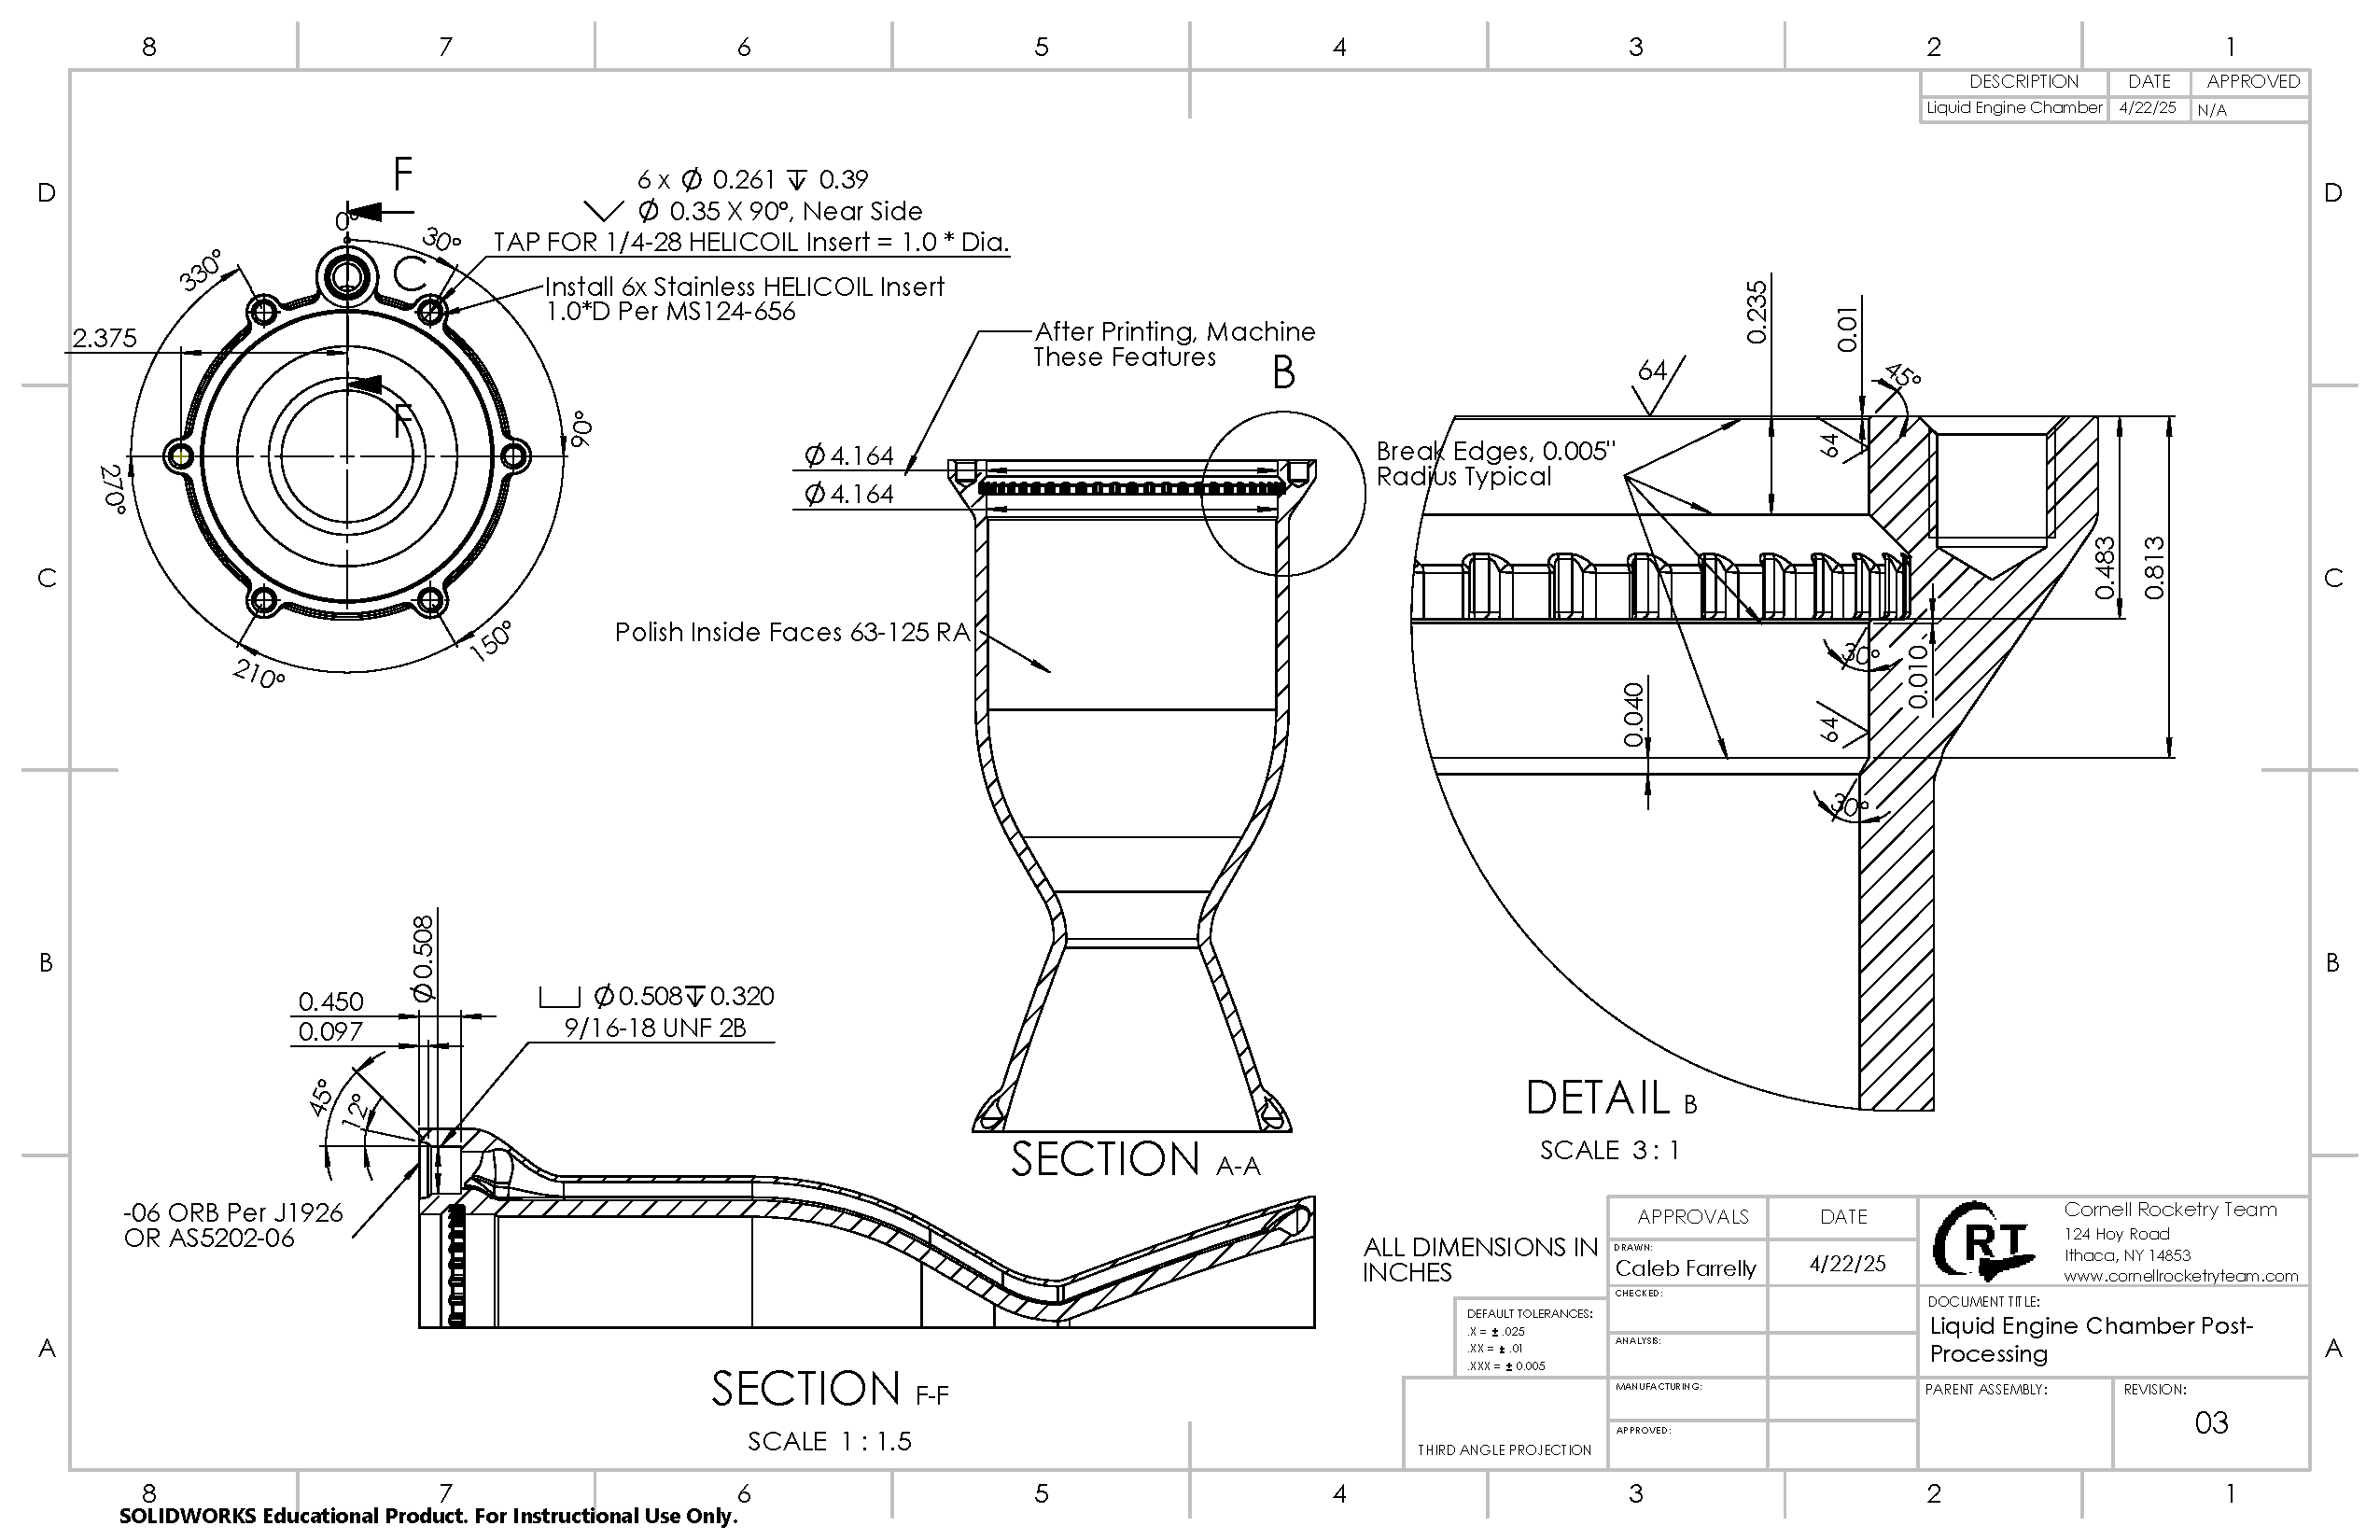
\includepdf[pages=-,fitpaper]
{ReportSections/Liquid_Engine_Chamber_Post_Processing_Rev3.PDF}

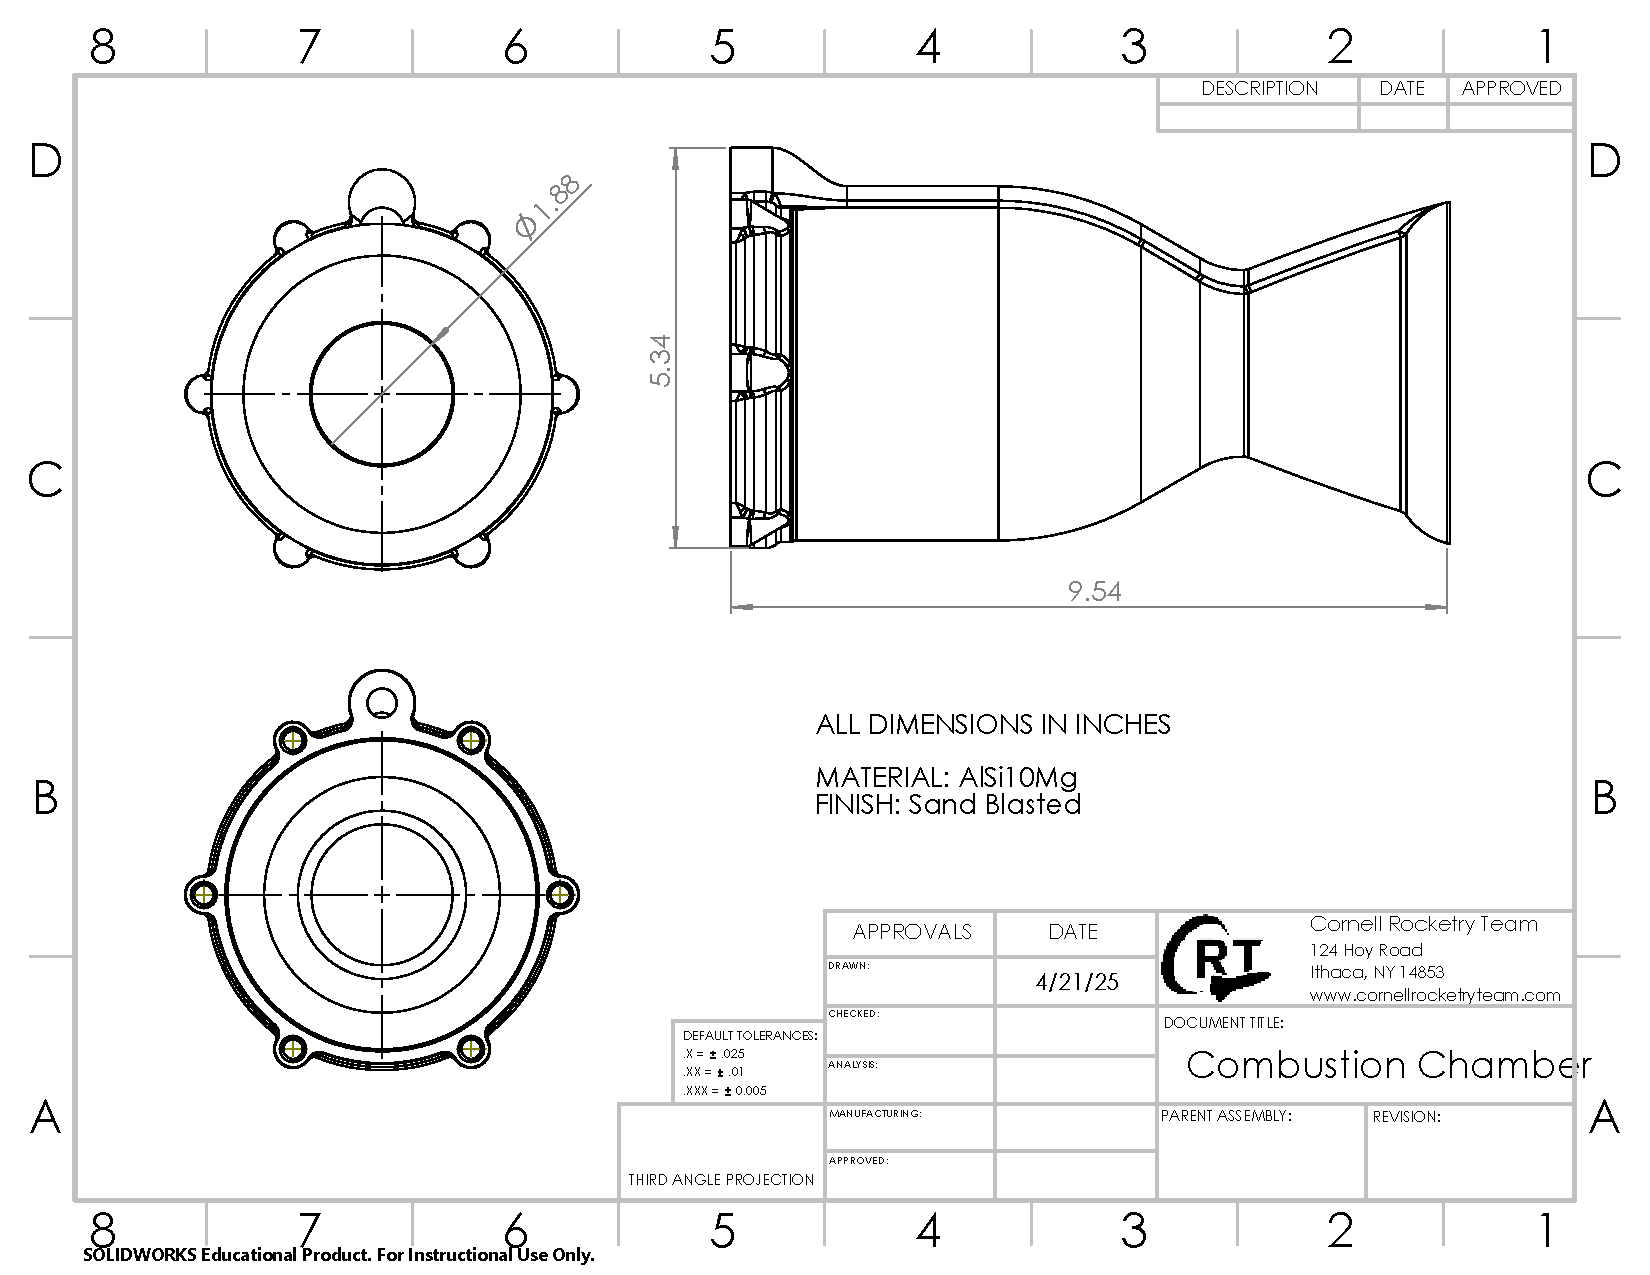
\includepdf[pages=-,fitpaper]
{ReportSections/CRT_Liquid_Engine_Chamber_for_Print.PDF}

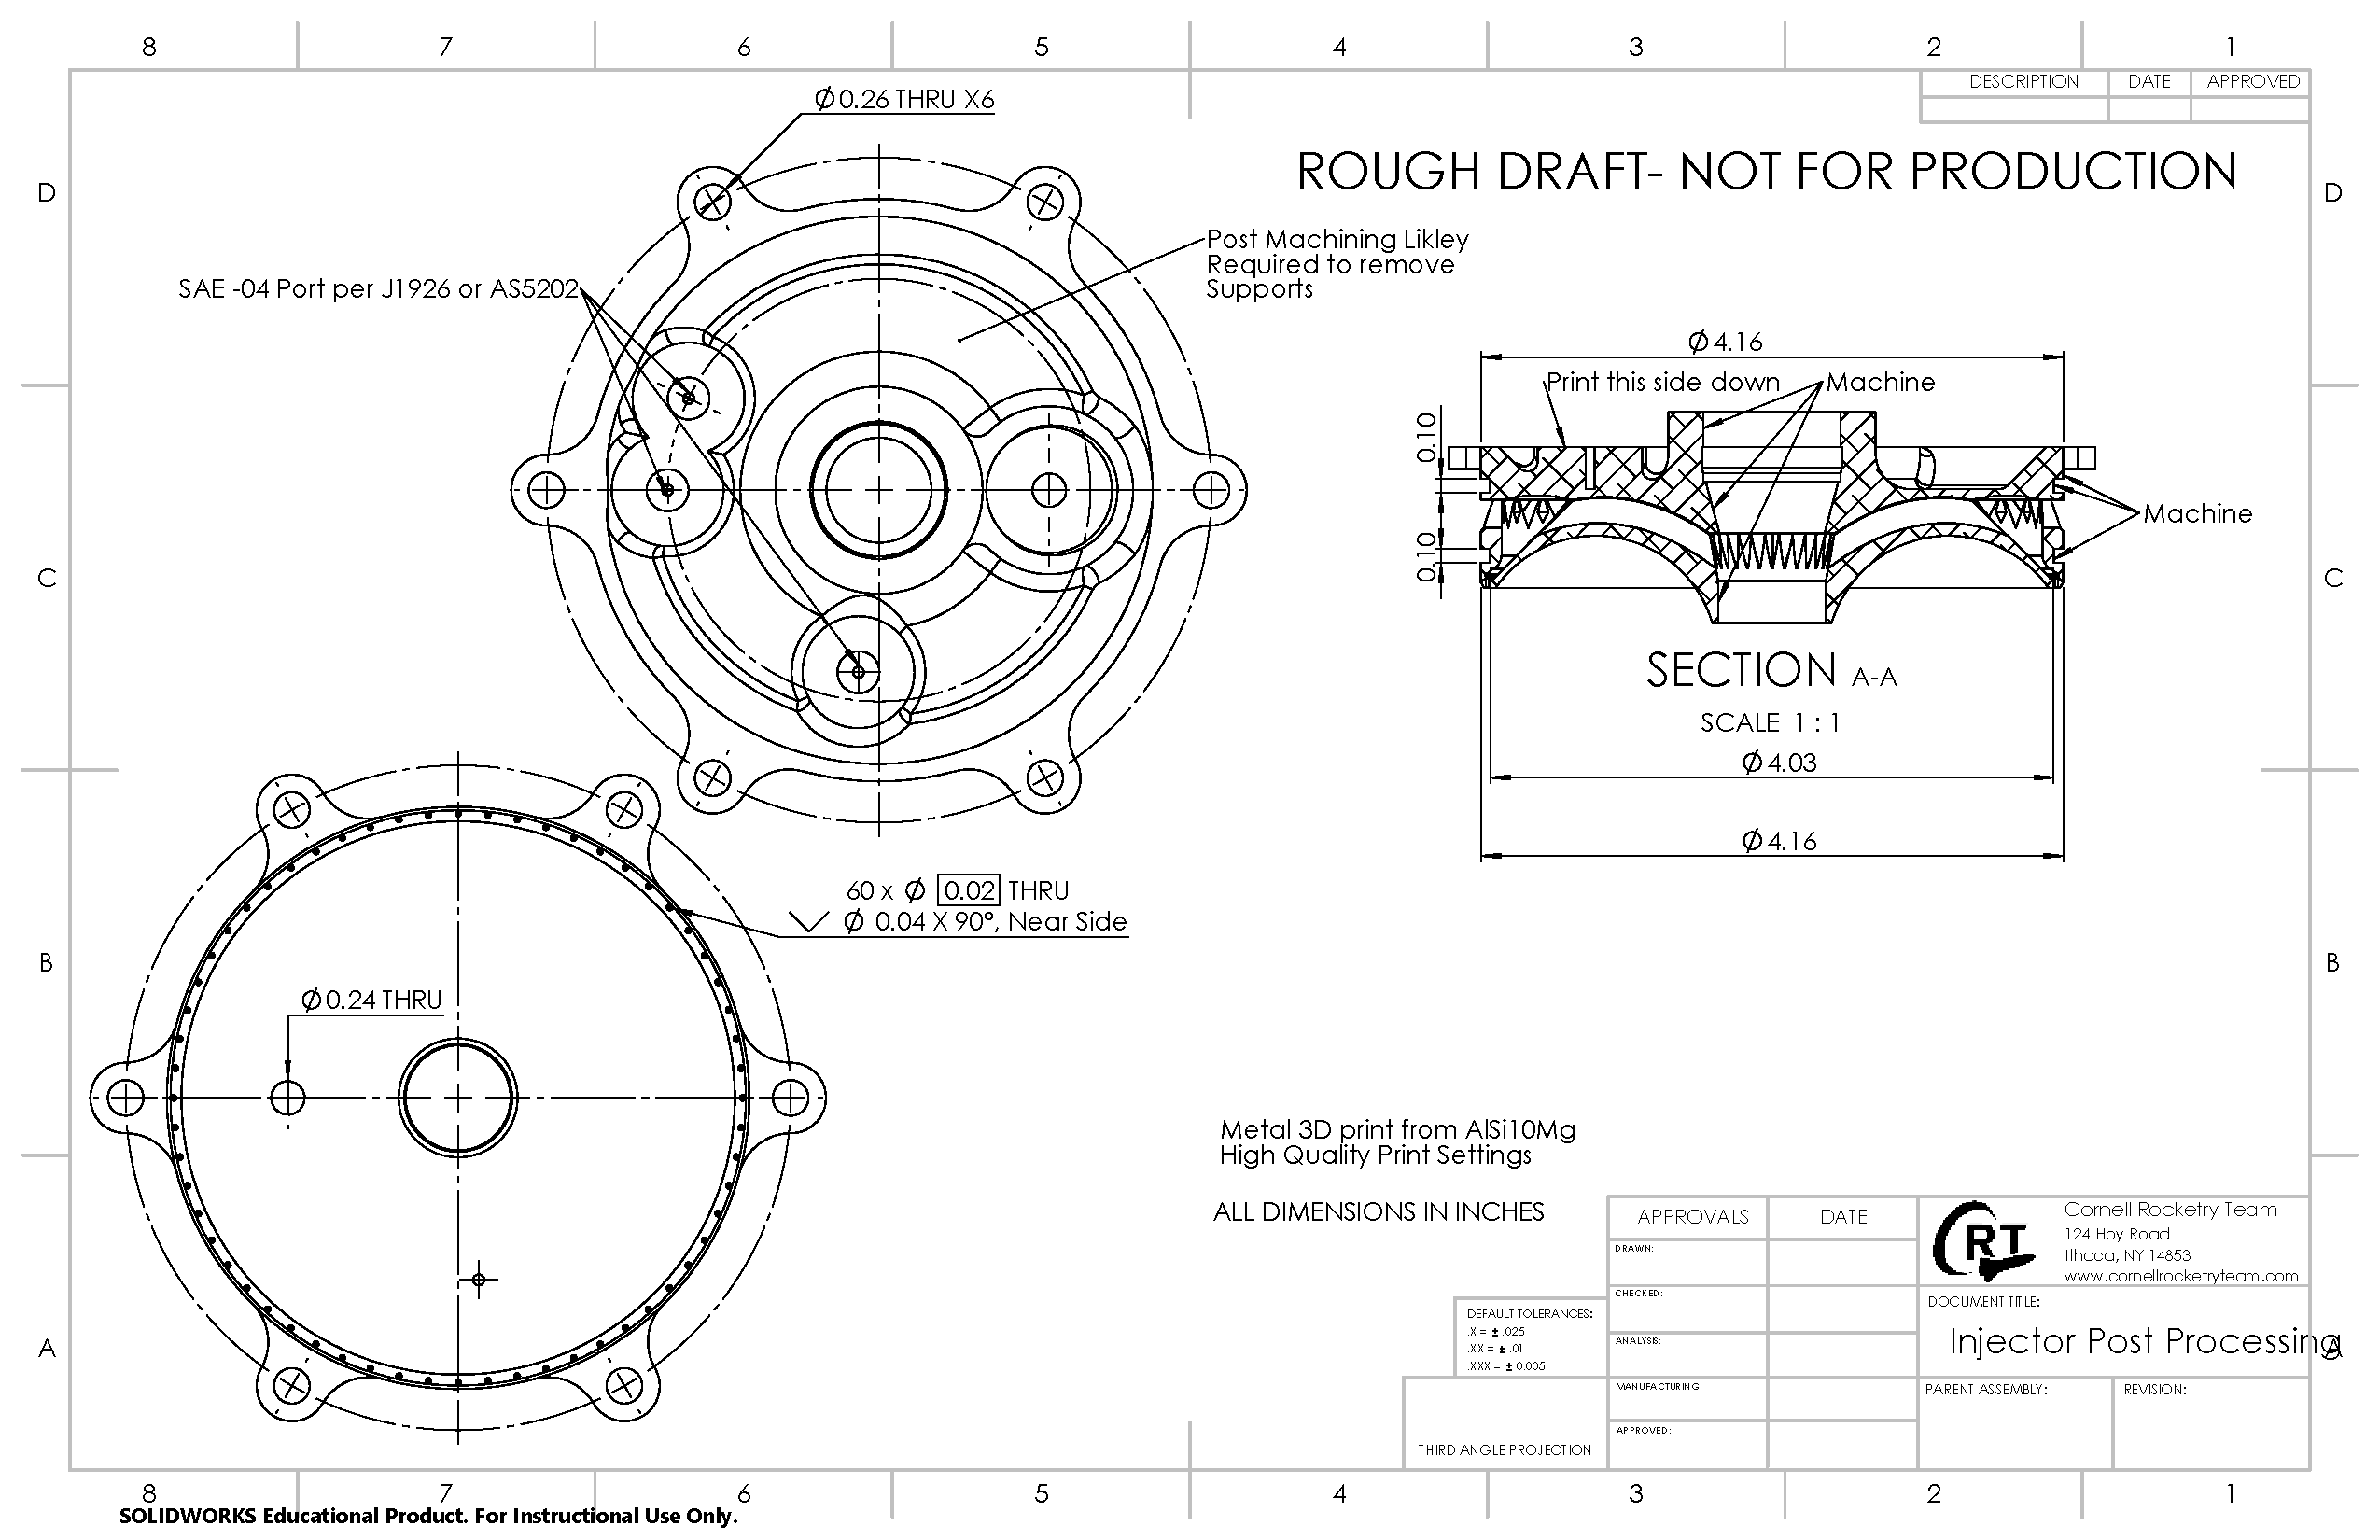
\includepdf[pages=-,fitpaper]
{ReportSections/injectorbody3DP_Post_Machining.pdf}



\section{MATLAB Scripts for Engine Analysis}

This appendix contains the MATLAB scripts used for various calculations related to the design of the 1250 lbf bipropellant rocket engine. These scripts include fuel flow calculations, cooling channel analysis, and structural stress analysis.


\begin{minted}[breaklines,fontsize=\small]{matlab}
clc; clear;

% === Input Parameters ===
% === Ethanol Flow Through Annular Orifice ===
% Given Data
Cd = 0.82;                % Discharge coefficient
rho = 780;                % Density of ethanol (kg/m^3)

% Orifice Inner Diameter in Inches (Given)
d_inner_in = 0.74525;     % Inner diameter of orifice (inches)

% Desired Mass Flow Rate in kg/s
desired_mass_flow_kg_s = 0.68;  % Desired mass flow rate (kg/s)

% Pressure in PSI
P1_psi = 700;             % Upstream pressure (PSI)
P2_psi = 350;             % Downstream pressure (PSI)

% Convert Units
P1 = P1_psi * 6894.76;    % Upstream pressure (Pa)
P2 = P2_psi * 6894.76;    % Downstream pressure (Pa)
deltaP = P1 - P2;         % Pressure drop (Pa)
d_inner = d_inner_in * 0.0254;  % Inner diameter in meters

% Solve for Pintle Gap
syms pintle_gap
d_outer = d_inner + 2 * pintle_gap;  % Outer diameter in meters
A = pi * (d_outer^2 - d_inner^2) / 4;  % Annular area (m^2)

% Flow Equation: Mass Flow Rate = rho * Cd * A * sqrt(2 * deltaP / rho)
Q_m3s = Cd * A * sqrt(2 * deltaP / rho); % Volumetric flow rate (m^3/s)
mass_flow_eq = rho * Q_m3s;              % Mass flow rate (kg/s)

% Solve for Pintle Gap
solution = vpasolve(mass_flow_eq == desired_mass_flow_kg_s, pintle_gap);
solution = max(solution); % Take the first valid solution
pintle_gap_in = double(solution / 0.0254);  % Convert to inches

% Display Results
fprintf('Ethanol Flow Through Annular Orifice:\n');
fprintf(' - Desired Mass Flow Rate: %.2f kg/s\n', desired_mass_flow_kg_s);
fprintf(' - Pressure Drop: %.2f PSI\n', P1_psi - P2_psi);
fprintf(' - Pintle Gap: %.6f m (%.6f inches)\n', double(solution), pintle_gap_in);

% === Cooling Calculations ===
% Chamber Data
chamber_flux = 3.2574;   % Chamber mass flux (kg/s) from RPA
cooling_fraction = 0.053; % Fraction of fuel for film cooling
fuel_injector_mdot = 0.6786; % Fuel mass flow rate from injector (kg/s)

% Coolant Mass Flow Rate
cool_film_mdot = cooling_fraction * chamber_flux;  
total_fuel_mass_flow_rate = fuel_injector_mdot + cool_film_mdot;  

% Percent of Fuel Used for Regenerative Cooling
percent_regen = total_fuel_mass_flow_rate / chamber_flux;  

% === Fluid Properties of Ethanol ===
mu = 0.001095;    % Dynamic viscosity (Pa·s) at ~20°C
epsilon = 60e-6;  % Aluminum surface roughness for 3D printing (m)

% === Cooling Channel Geometry ===
channel_length = 0.25;    % Channel length (m)
num_channels = 58;        % Number of cooling channels
A_channel = 2.66291e-6;   % Cross-sectional area per channel (m^2)
P = 5.938e-3;             % Perimeter from CAD model (m)

% Perimeter was calculated by taking the cross-section of the cooling
% channels at the smallest area, around the throat. Smaller channels at the throat 
% increase flow velocity, enhancing heat transfer from the walls to the fluid.

% Calculate Hydraulic Diameter
D_h = 4 * (A_channel / P);  

% Calculate Flow Velocity
Q = total_fuel_mass_flow_rate / (rho * num_channels);  
v = Q / A_channel;    

% Calculate Reynolds Number
Re = (rho * v * D_h) / mu;

% === Friction Factor Calculation ===
if Re < 2300
    f = 64 / Re;  % Laminar flow
elseif Re >= 4000
    % Turbulent flow using Colebrook-White equation
    syms f_sym
    colebrook_eq = -2 * log10((epsilon/(3.7*D_h)) + (2.51/(Re*sqrt(f_sym)))) == 1/sqrt(f_sym);
    f = double(vpasolve(colebrook_eq, f_sym, 0.02)); 
else
    % Transitional flow (Blasius approximation)
    f = 0.079 * Re^(-0.25); 
end

% Calculate Pressure Drop Using Darcy-Weisbach Equation
deltaP_Pa = f * (channel_length / D_h) * (rho * v^2 / 2);  % Pressure drop (Pa)
deltaP_PSI = deltaP_Pa / 6894.76;  % Pressure drop (PSI)

% === Orifice Calculations for Film Cooling ===
% Film coolant mass flow rate
orifice_diameter = 0.4e-3;  % Orifice diameter (m)
Cd_orifice=0.6; %typical sharp edged orifice 
A_orifice = pi * (orifice_diameter / 2)^2;  % Orifice cross-sectional area (m^2)

% Flow Rate Through One Orifice
syms orifice_mdot
orifice_eq = rho * Cd * A_orifice * sqrt(2 * deltaP / rho) == orifice_mdot;
orifice_mdot_sol = double(vpasolve(orifice_eq, orifice_mdot));

% Calculate Number of Orifices
num_orifices = ceil(cool_film_mdot / orifice_mdot_sol);

% === Display Results ===
fprintf('\nCooling and Flow Results:\n');
fprintf(' - Total Fuel Mass Flow Rate: %.2f kg/s\n', total_fuel_mass_flow_rate);
fprintf(' - Reynolds Number: %.2f\n', Re);
fprintf(' - Flow Velocity: %.2f m/s\n', v);
fprintf(' - Friction Factor: %.4f\n', f);
fprintf(' - Pressure Loss: %.4f Pa (%.4f PSI)\n', deltaP_Pa, deltaP_PSI);
fprintf(' - Film Coolant Mass Flow Rate: %.6f kg/s\n', cool_film_mdot);
fprintf(' - Orifice Flow Rate: %.6f kg/s per orifice\n', orifice_mdot_sol);
fprintf(' - Number of Orifices Required: %d\n', num_orifices);

% Determine Flow Regime
if Re < 2300
    fprintf(' - Flow Regime: Laminar\n');
elseif Re <= 4000
    fprintf(' - Flow Regime: Transitional\n');
else
    fprintf(' - Flow Regime: Turbulent\n');
end


% Cooling Channel Stress Analysis 
clc; clear;

% Constants and Inputs
pc = 350 * 6895;    % Chamber pressure (Pa) from psi
fp = 1000 * 6895;   % Fuel MEOP (Pa) from psi
t = 0.0015;         % Cooling channel min wall thickness (m)
ri = 0.046;         % Inner radius of the cooling channel (m)
sf = 1.5;           % Safety factor
yall = 125e6;       % Allowable material yield strength (Pa) at 250c for EOS EOS Aluminium AlSi10Mg 

% Cooling Channel Inside Stress
rcooling = 0.0015;    % Cooling channel width (m)
sigcool = (pc * sf * rcooling / t) / 1e6;  % Cooling channel stress (MPa)
margincool = (yall / (sig * 1e6)) - 1; % Safety margin


% Fuel distribution manifold stress calculation
ptank = 800 * 6895;   % Fuel tank pressure (Pa)
sig = (pc * sf * ri / t) / 1e6;   % Main wall stress (MPa)
margin = (yall / (sig * 1e6)) - 1; % Safety margin

% Cooling Mass Flux Calculations
coolf = 0.053;               % Cooling mass fraction
chamberflux = 3.2574;        % Chamber flux (kg/s)
coolmflux = coolf * chamberflux; % Cooling mass flux (kg/s)
fuel = 0.6786;               % Base fuel flow (kg/s)
totalfuel = fuel + coolmflux; % Total fuel flow (kg/s)
percentregen = totalfuel / chamberflux; % Regen fuel percentage



% Convert wall thickness to thousandths of an inch
thou = t * 1000 * 39.37; % Wall thickness in thousandths of an inch

% Cooling Channel Pressure Data
pout = 6.1629; % Outlet pressure (MPa)
pin = 6.20528;  % Inlet pressure (MPa)
dpcool = (pin - pout) * 145; % Pressure drop in cooling channel (psi)

% Display Results
fprintf('Structural and Flow Analysis Results:\n');
fprintf(' - Cooling Channel Stress: %.2f MPa\n', sigcool);
fprintf(' - Main Wall Stress: %.2f MPa\n', sig);
fprintf(' - Safety Margin: %.2f%%\n', margin * 100);
fprintf(' - Total Fuel Flow: %.4f kg/s\n', totalfuel);
fprintf(' - Regen Fuel Percentage: %.2f%%\n', percentregen * 100);
fprintf(' - Cooling Channel Pressure Drop: %.2f psi\n', dpcool);
fprintf(' - Wall Thickness: %.2f thou\n', thou);
\end{minted}